\documentclass[oneside,a4paper,12pt]{book}
\usepackage[american]{babel}
%\pagestyle{headings}
\frontmatter

%=============================================================================

\usepackage{amsthm}
\usepackage{xspace}
\usepackage{float}
\usepackage{ifthen}
\usepackage{amsbsy}
\usepackage{amssymb}
\usepackage{balance}
\usepackage{booktabs}
\usepackage{graphicx}
\usepackage{rotating}
\usepackage{multirow}
\usepackage{needspace}
\usepackage{microtype}
\usepackage{bold-extra}
\usepackage{geometry}
\usepackage{varioref}
\usepackage{xcolor}
\usepackage{textcomp}
\usepackage{listings}
\usepackage[normalem]{ulem} %emphasize still italic
\usepackage{ucs}
\usepackage{array}

% \usepackage[utf8]{inputenc}
% \usepackage[htt]{hyphenat}
\usepackage{times}
\usepackage{url}
\usepackage{alltt}
\usepackage{amsmath}
\usepackage{xfrac}
\usepackage{subfigure}
\usepackage{appendix}
\usepackage{stmaryrd}   % for the \shortuparrow
\usepackage[utopia]{quotchap}

\usepackage{setspace}
\usepackage[numbers, sort&compress]{natbib}
\usepackage{mdwlist}        % support for better spaced lists
% allows for temporary adjustment of side margins
\usepackage{chngpage}
\usepackage[normalem]{ulem} 

% constants

\newcounter{qcounter}

% commands
\newcommand{\n}{$\cdot$}
\newcommand{\y}{\checkmark}
\newcommand{\subscript}[1]{$_{\textrm{\footnotesize{#1}}}$}
\newcommand{\superscript}[1]{$^{\textrm{\footnotesize{#1}}}$}
\newcommand{\vertical}[1]{\raisebox{-4em}{\begin{sideways}{#1}\end{sideways}}}

\newboolean{showedits}
\setboolean{showedits}{true} % toggle to show or hide edits
\ifthenelse{\boolean{showedits}}
{
       \newcommand{\ugh}[1]{\textcolor{red}{\uwave{#1}}} % please rephrase
       \newcommand{\ins}[1]{\textcolor{blue}{\uline{#1}}} % please insert
       \newcommand{\del}[1]{\textcolor{red}{\sout{#1}}} % please delete
       \newcommand{\chg}[2]{\textcolor{red}{\sout{#1}}{\ra}\textcolor{blue}{\uline{#2}}} % please change
}{
       \newcommand{\ugh}[1]{#1} % please rephrase
       \newcommand{\ins}[1]{#1} % please insert
       \newcommand{\del}[1]{} % please delete
       \newcommand{\chg}[2]{#2}
}


% ============================================================================
% Put edit comments in a really ugly standout display

\usepackage{xcolor}
\usepackage[normalem]{ulem}
\newcommand{\ra}{$\rightarrow$}


% comments \nb{label}{color}{text}
\newboolean{showcomments}
\setboolean{showcomments}{true}
\ifthenelse{\boolean{showcomments}}
    {\newcommand{\nb}[3]{
        {\colorbox{#2}{\bfseries\sffamily\scriptsize\textcolor{white}{#1}}}
        {\textcolor{#2}{\sf\small$\blacktriangleright$\textit{#3}$\blacktriangleleft$}}}
     \newcommand{\version}{\emph{\scriptsize$-$Id$-$}}
%	 \newcommand{\ugh}[1]{\textcolor{red}{\uwave{#1}}} % please rephrase
%	 \newcommand{\ins}[1]{\textcolor{blue}{\uline{#1}}} % please insert
%	 \newcommand{\del}[1]{\textcolor{red}{\sout{#1}}} % please delete
%	 \newcommand{\chg}[2]{\textcolor{red}{\sout{#1}}{\ra}\textcolor{blue}{\uline{#2}}} % please change
	 \newcommand{\chk}[1]{\textcolor{ForestGreen}{#1}} % changed, please check
	}
    {\newcommand{\nb}[3]{}
     \newcommand{\version}{}
	\newcommand{\chk}[1]{} % changed, please check
	}

% ============================================================================
% Make quotes be italic
\renewenvironment{quote}
    {\list{}{\rightmargin\leftmargin}%
     \item\relax\begin{it}}
    {\end{it}\endlist}

\newcommand{\ttimes}{\ensuremath{\times}}

%=============================================================================

\newcommand{\needlines}[1]{\Needspace{#1\baselineskip}}

% source code
\usepackage{xcolor}
\usepackage{textcomp}
\usepackage{listings}
\definecolor{source}{gray}{0.9}
\lstset{
	language={},
	% characters
	tabsize=3,
	upquote=true,
	escapechar={!},
	keepspaces=true,
	breaklines=false,
	alsoletter={:},
	breakautoindent=true,
	columns=fullflexible,
	showstringspaces=false,
	basicstyle=\footnotesize\ttfamily,
	% background
	frame=single,
    framerule=0pt,
	backgroundcolor=\color{source},
	% numbering
	numbersep=5pt,
	numberstyle=\tiny,
	numberfirstline=true,
	% captioning
	captionpos=b,
	numberbychapter=false,
	% formatting (html)
	moredelim=[is][\textbf]{<b>}{</b>},
	moredelim=[is][\textit]{<i>}{</i>},
	moredelim=[is][\uline]{<u>}{</u>}}
\newcommand{\ct}{\lstinline[backgroundcolor=\color{white},basicstyle=\footnotesize\ttfamily]}
\newcommand{\lct}[1]{{\small\tt #1}}


%----------------------------------------------------------------------------
% references
\newcommand{\tabref}[1]{\hyperref[{tab:#1}]{Table~\ref*{tab:#1}}}
\newcommand{\figref}[1]{\hyperref[{fig:#1}]{Figure~\ref*{fig:#1}}}
\newcommand{\secref}[1]{\hyperref[{sec:#1}]{Section~\ref*{sec:#1}}}
\newcommand{\lstref}[1]{\hyperref[{lst:#1}]{Listing~\ref*{lst:#1}}}
\newcommand{\charef}[1]{\hyperref[{cha:#1}]{Chapter~\ref*{cha:#1}}}
%----------------------------------------------------------------------------

% abbreviations
\tracingcolors 4
\setcounter{tocdepth}{3}
\setcounter{secnumdepth}{3}
\newcommand{\ie}{\emph{i.e.,}\xspace}
\newcommand{\eg}{\emph{e.g.,}\xspace}
\newcommand{\etc}{\emph{etc.}\xspace}
\newcommand{\etal}{\emph{et al.}\xspace}


\newcommand{\newevenside}{
	\ifthenelse{\isodd{\thepage}}{\newpage}{
	\newpage
        \phantom{placeholder} % doesn't appear on page
	\thispagestyle{empty} % if want no header/footer
	\newpage
	}
}

\def\stretchfactor{1}
\newcommand{\mychapter}[1]{\setstretch{1}
    \chapter{#1}\setstretch{\stretchfactor}}

%----------------------------------------------------------------------------
\newcommand{\lessSpace}{\vspace{-1em}}
\DeclareGraphicsExtensions{.pdf,.png}
\graphicspath{{images/}}
\newcommand{\fig}[4]{
	\begin{figure}[#1]
		\centering
		\includegraphics[width=#2\textwidth]{#3}
		\lessSpace
		\caption{\label{fig:#3}#4}
	\end{figure}}

% ===========================================================================

%:CONFIGURE THIS

\newcommand{\thesistitle}{Cryptographic APIs}
\newcommand{\thesisauthor}{Sophie Gabriela Pfister}
\newcommand{\thesisauthorOrigin}{Bern, Switzerland}
\newcommand{\thesisleiter}{Prof.\ Dr.\ Oscar Nierstrasz}
\newcommand{\thesisasst}{Dr.\ Mohammad Ghafari, Mohammadreza Hazhirpasand}
\newcommand{\thesisurl}{http://scg.unibe.ch/}
\newcommand{\thesissubtitle}{Evaluating the Usability of Java Cryptography Architecture}
\newcommand{\thesisdate}{31. Dezember 2021}

% ===========================================================================

\usepackage[ colorlinks=true, urlcolor=black, linkcolor=black,
			citecolor=black, bookmarksnumbered=true, bookmarks=true,
			plainpages=false,
			pdftitle={\thesistitle}, pdfauthor={\thesisauthor},
			pdfsubject={\thesissubtitle}, pdfpagelabels]{hyperref}

\newcommand{\hrref}[2]{\hyperref}
% ===========================================================================
% ===========================================================================

\hypersetup{
    colorlinks=true,
    linkcolor=black,
    filecolor=magenta,      
    urlcolor=blue,
    }

% D O C U M E N T
% % % % % % % % % % % % % % % % % % % % % % % % % % % % % % % % % %
\begin{document}

% T I T L E
% % % % % % % % % % % % % % % % % % % % % % % % % % % % % % % % % %
\begin{titlepage}  
  \begin{center}  
  
  \begin{figure}[t]  
  \vspace*{-2cm}        % to move header logo at the top 
  \center{
\includegraphics[scale=0.5]{logos/UNI_Bern.png}}
  \vspace{1.2in}     
  \end{figure}

    \thispagestyle{empty}
    
    {\bfseries\Huge \thesistitle \par
    \Large \vspace{0.1in} \thesissubtitle \par}

    \vspace{0.3in} 
    \LARGE{\textbf{Bachelor Thesis} \\}
    \vspace{0.4in}

    {\Large \thesisauthor \par from \par \thesisauthorOrigin}
    
    \vspace{0.3in}
    {\Large Philosophisch-naturwissenschaftlichen Fakult\"{a}t \\
            der Universit\"{a}t Bern \par}
    \vspace{0.3in}
    {\Large \thesisdate \par}
    \vspace{0.3in}
    %Leiter der Arbeit: \par
   {\Large \thesisleiter} \par
      {\Large \thesisasst} \par
   \vspace{0.1in}
    {\Large Software Composition Group \par Institut f\"{u}r Informatik \par University of Bern, Switzerland \par}
  

  %\vspace{0.5in}
 
 

  \end{center}

\end{titlepage}


% A B S T R A C T
% % % % % % % % % % % % % % % % % % % % % % % % % % % % % % % % % %
\chapter*{\centering Abstract}
\begin{quotation}
\noindent 
% ToDo: Abstract
\end{quotation}
\clearpage


% C O N T E N T S 
% % % % % % % % % % % % % % % % % % % % % % % % % % % % % % % % % % % % % % % %
\tableofcontents

\mainmatter
%%%%%%%%%%%%%%%%%%%%%%%%%%%%%%%%%%
%%%% NEW CHAPTER %%%%%%%%%%%%%%%%%%%%%
%%%%%%%%%%%%%%%%%%%%%%%%%%%%%%%%%%

% === I N T R O D U C T I O N ===
\chapter{Introduction}
\label{cha:Introduction}
% === Relevance of Cryptography  & Cryptographic APIs + Issues ===
Cryptography is a fundamental part of our digital world. 
It provides techniques to ensure confidentiality, authenticity, and integrity of information. 
Yet, Buchanan described the internet as an unsafe place \cite{buchanan2017}. 
He complained that too little security was implemented in the services and protocols used. 
He insisted that "the next generation of the Internet [...] must be built in a trustworthy way" (Buchanan, 2017, \cite{buchanan2017}, p. 1).\\
In practice, we witness a large number of vulnerabilities found in various software and protocols each year.\footnote{http://www.exploit-db.com}
One of the disastrous weakness types is the ones concerning cryptography. 
Although there exist a great number of cryptography libraries for building secure applications by providing services such as hashing, symmetric, and asymmetric encryption, a series of recent studies have indicated that software developers have difficulty using cryptography correctly.
Krüger \etal found at least one misuse of a cryptography API in 96\% of 10'001 investigated Android applications \cite{kruger2017}.
Piccolboni \etal analyzed the 1780 most popular free apps from Google Play Store that make use of cryptography APIs and found that more that 99.7\% used inappropriate sources for random number generation and 99.1\% used broken hash functions \cite{piccolboni2020}.\\
\par
One of the leading issues is that cryptography libraries lack usability. 
This issue has been studied in a number of well-known cryptography libraries. 
The results showed that libraries often do not support auxiliary tasks (\ie Mindermann \etal \cite{mindermann2018}),  that they are not abstract enough (\ie Nadi \etal \cite{nadi2016}), and that they lack documentation quality (\ie Mindermann \etal \cite{mindermann2018}, Nadi \etal \cite{nadi2016}, Patnaik \etal \cite{patnaik2019}).
Similarly, the results of Acar \etal imply that unusable cryptography libraries do not only prevent developers from writing functional code but also lead to the emergence of security vulnerabilities since developers are more likely to misuse APIs \cite{acar2017}.
What's more, a good documentation is a strong predictor for both, functional and secure code.
Acar \etal emphasized the importance of having an official documentation, which contains secure examples "to keep developers from searching for unvetted, potentially insecure alternatives" (2017, \cite{acar2017}, p.167).\\

% === Project Goals & Research Questions ===
\par
We believe that still some areas, such as context of API usability, documentation usability, API misuse and unsafe code, need closer investigations. 
Therefore, for the three aforementioned areas, we are interested to address the following research questions:
\begin{enumerate}
	\item What issues do programmers face when implementing symmetric encryption using Java Cryptography Architecture?
	\item What security risks can be found in code and advises shared on Stack Overflow referring to the implementation of symmetric encryption scenarios Java Cryptography Architecture?
	\item To what extent are these issues linked to missing or inadequate documentation?
\end{enumerate}

Since different cryptography libraries have different API design, it may manifest various and scattered types of issues if we had studied more than one cryptography libraries on Stack Overflow. 
As a result, we focused on one library (\ie Java Cryptography Architecture) and one use case (\ie symmetric encryption) to gain a deeper understanding of the issues, which provides us with more details compared to previous research that focused on a more general level.
The Java Cryptography Architecture (JCA) has been examined in recent studies, \ie Nadi \etal \cite{nadi2016} and Hazhirpasand \etal \cite{hazhirpasand2020}.
Moreover, JCA is the default cryptography API for Java developers and acquired FIPS-140 standards issued by the National Institute of Standards and Technology (NIST) to specify the requirements for cryptography libraries and modules. \footnote{\href{https://nvlpubs.nist.gov/nistpubs/FIPS/NIST.FIPS.140-3.pdf}{FIPS-140-3}}\\

% === Methodology ===
\par
To answer our research questions, we analyzed 150 threads from Stack Overflow where at least one issue related to our scope was discussed.
We used three queries and computed the sample size per query proportional to the number of posts returned by it.
We also selected half of the sample from the newest threads and the other half from the most popular ones.
To answer the first research question, we identified the issues the person asking the question (original poster) was facing and categorized them regarding technical aspects or requirements that have not been met.
To answer the second research question, we checked the same sample for rule violations based on a predefined set of security rules for symmetric encryption scenarios.
To answer the third research question, we derived a set of prioritized questions from the previous findings and sought their answer in the documentation of JCA library.
We also took notes regarding documentation quality in general.\\

% === Results ===
\par
Our key findings were that programmers struggled most with properly handling keys, encryption modes\footnote{cipher block mode of operation}, and initialization vectors. 
This was found regarding both, the first and the second research question.
Regarding the first research question, we also observed that developers failed to correctly configure dependencies between different properties.
They also struggled with the API design of JCA, especially the dependency from providers and various method overloads.
We also found more evidence that programmers lack domain knowledge to successfully implement symmetric encryption.\\
Regarding the second research question, we found that programmers frequently used unsafe encryption modes (ECB, CBC).
The code snippets on Stack Overflow also made use of static values for keys and initialization vectors.
Furthermore, password based key derivation was sometimes not implemented in a secure way.\\
Regarding the third research question, observed that most of the derived questions were covered by the documentation, especially the ones with higher priorities.
We concluded that most of the issues could have been prevented if the original poster thoroughly read and understood the documentation.
Yet, we issued some recommendations to improve it.\\


% === Thesis Structure ===
\par
In this thesis, we first present the state of research in chapter \ref{cha:RelWo}. 
In chapter \ref{cha:Method}, we describe the methodical approaches of our study. 
We explain and interpret our results in chapter \ref{cha:Results}.
Chapter \ref{cha:Conclusion} includes the conclusion, limitations, and conductive thoughts.
In the "Anleitung zum Wissenschaftlichen Arbeiten" (chapter \ref{cha:AWI}), we describe Mayring's guidelines for qualitative content analysis more precisely that were followed during our analyses.

% === R E L A T E D   W O R K ===
\chapter {Related Work}
\label{cha:RelWo}


% === Usability ===
\section{API Usability}
\label{cha:ApiUsability}
One of the most popular definitions for usability is the one by ISO 92411-11:1998: "the extent to which a product can be used by specified users to achieve specified goals with effectiveness, efficiency and satisfaction in a specified context of use" (ISO 9241-11, \cite{iso1998}, p.2).
Although the definition is very precise, it does not explain how to measure the usability of a product.\\
\par
Past research on (API) usability approached the topic in different ways and the literature is therefore rather heterogeneous.
Some researchers focused rather on programmers' needs and defined guidelines and heuristics to describe what a usable API should look like. 
Zibran conducted a meta analysis on API usability literature and described a set of 22 specific guidelines \cite{zibran2008}.
He considered an API as usable if it was "(1) easy to learn, (2) easy to remember, (3) easy write client code, (4) easy to interpret client code, and (5) difficult to misuse" (2008, \cite{zibran2008}, p. 256).\\
Other researchers approached the problem from the perspective of software metrics.
Rama \& Kak proposed 8 metrics for API usability referring to method overloads and name confusion, method grouping, parameter list complexity and consistency, thread safety, and documentation \cite{rama2015}.
Scheller \& Kühn even defined an extensible framework to measure interface complexity automatically \cite{scheller2015}.\\
Another approach was to focus on the concept of usability and redefine it more precisely.
Alonso-Ríos \etal investigated the concept and described it using a detailed taxonomy \cite{alonso2010}.
Starting from usability, they organized a wide range of attributes in a hierarchy.\\

\par
Mosquiera-Rey \etal combined several approaches \cite{mosqueira2018}.
They extended the usability model by Alonso-Rìos \etal with the context of use and mapped existing guidelines for API usability to the model's attributes.
The first level attributes of those taxonomies are shown in figure \ref{fig:ApiUsability}.
They found and described a total of 45 heuristics for API usability.
\begin{figure}[h]
\centering
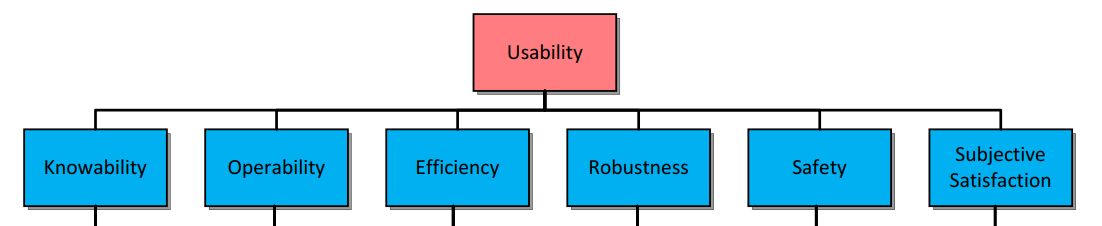
\includegraphics[width=0.65\textwidth]{ApiUsability}
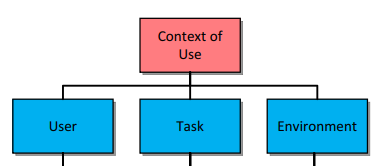
\includegraphics[width=0.33\textwidth]{ContextOfUse}
\caption{First Level Attributes of Usability and Context of Use Taxonomies (Mosquiera-Rey \etal, 2018, \cite{mosqueira2018}, p. 49 ff.)}
\label{fig:ApiUsability}
\end{figure}

% Documentation Usability
\section{Usability Criteria for Documentation}
Mosquiera-Rey \etal located documentation quality within the \emph{Knowability} attribute of an API \cite{mosqueira2018}.
They defined this property as the extent a programmer can "understand, learn, and remember how to use the system" (Mosquiera-Rey \etal, 2018, \cite{mosqueira2018}, p. 48).
They described three documentation related heuristics:
\begin{itemize}
	\item Documentation should not contain irrelevant information such as meta data or obsolete and redundant comments.
	\item Documentation should contain code samples for key scenarios.
	\item Documentation should identify deprecated methods, explain why these are deprecated, and propose alternatives.
\end{itemize}

Robillard asked developers what they struggled with most when they had to learn a new API \cite{robillard2009}.
Their answers identified missing or unclear documentation as a major obstacle.
Robillard concluded that API documentation must be complete and provide example code.
Additionally, it should support a wide range of usage scenarios, include relevant design elements, and be organized in a convenient way.\\

\newpage
% Recommendations for Crypto Documentation
\par
Mindermann \etal who evaluated the usability of rust cryptography libraries also made recommendations how to improve the usability of such libraries and their documentation \cite{mindermann2018}. 
These were more specific for the cryptographic context.
A good documentation for a cryptography API should additionally
\begin{itemize}
	\item link to comprehensible resources that explain cryptographic concepts.
	\item mention closely related keywords (\ie block cipher mode of operation, cipher mode, encryption mode).
	\item describe in which scenarios an algorithm should be used.
	\item warn from weaknesses and vulnerabilities (\ie unsafe algorithms that are supported for legacy).
	\item explain all parameters.
	\item give advise when there are multiple options and explain the differences between them.
\end{itemize}

\newpage
% Crypto API Usability
\section{Usability of Cryptography Libraries}
\label{cha:CryptoApi}

Green \& Smith defined ten principles regarding the usability and security of cryptography libraries \cite{green2016} .
Their key idea was that security-related functionalities should be integrated into non-cryptographic APIs such that regular programmers\footnote{without cryptography expertise} did not have to deal with cryptography APIs at all.
The entire set of principles is shown in figure \ref{fig:Princip}\\
\begin{figure}[h]
\centering
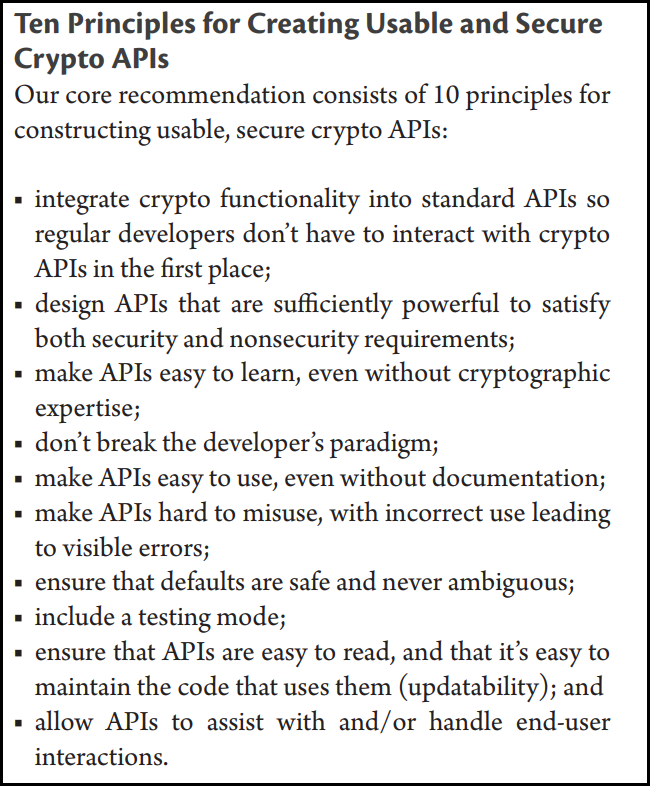
\includegraphics[width=0.65\textwidth]{GreenPrinciples}
\caption{10 Design Principles for Cryptography APIs by Green \& Smith (2016, \cite{green2016}, p. 42)}
\label{fig:Princip}
\end{figure}

\par
Patnaik \etal extended these principles by defining usability smells \cite{patnaik2019}.
They were looking for "telltale signs, that one of the ten usability principles is being violated" (2019, \cite{patnaik2019}, p. 245).
They examined a wide range of popular cryptography APIs: OpenSSL, NaCl, libsodium, Bouncy Castle, SJCL, Crypto-JS, and PyCrypto.
They manually reviewed almost 2500 posts on Stack Overflow and tried to identify the issues the programmers were facing.
They identified 16 thematic issues of which 2 related to the programmers' lack of knowledge:
\begin{itemize}
	\item \emph{Passing the buck}: Questions on Stack Overflow that are answered in documentation.
	\item \emph{Lack of Knowledge}: Questions implying that "the developer does not have foundation level cryptography knowledge" (Patnaik \etal, 2019, \cite{patnaik2019}, p. 250).
\end{itemize}
They mapped the remaining issues to four usability smells:\\
\begin{figure}[h]
\centering
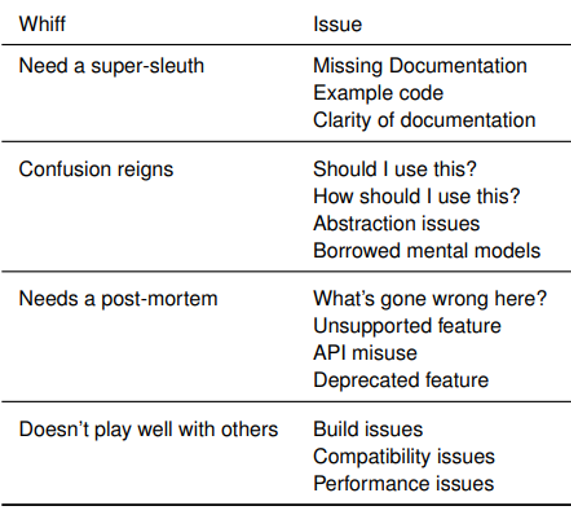
\includegraphics[width=0.6\textwidth]{UsabilitySmells}
\caption{Usability Smells and Issues as defined by Patnaik \etal (2019, \cite{patnaik2019}, p. 254)}
\label{fig:Smells}
\end{figure}

\par
Acar \etal also evaluated and compared five cryptography libraries for python \cite{acar2017}.\footnote{cryptography.io, Keyczar, PyNaCl, M2Crypto, and PyCrypto}
Their aim was to understand the reasons for failure (or success) when implementing cryptography scenarios and to define a blueprint for a new, more usable cryptography libraries.
They conducted a between-subjects online study where python programmers had to implement a symmetric or asymmetric encryption task using an assigned library.
Both, task and library, were assigned randomly.
The programmers also had to fill out an exit survey where they were asked about their backgrounds as well as their opinion regarding the assigned task and library.
Acar \etal then examined the submitted code regarding functionality and security and controlled their findings for the participant's background.\\
They found that the strongest predictors for working code was the documentation quality and the availability of working code examples.
When it comes to security, the programmers background was most important. Developers with a security background were more likely to produce secure code.
Although "simpler" APIs\footnote{more abstract, secure default values} seemed to promote better security results, they did not completely solve security problems.
The key issues regarding security were that libraries did not support auxiliary tasks (\ie key storage) and lacking documentation quality.
Acar \etal also observed that a complex API with good documentation (\ie PyCrypto) was rated more usable than a simple API with bad documentation (\ie Keyczar) by the participants.\\

\par
Mindermann \etal evaluated the usability of Rust cryptography libraries \cite{mindermann2018}.
After determining the most popular libraries, they conducted an exploratory study where one of the authors completed a set of cryptography related task several times using a different library for each round.
They afterwards compared two popular libraries, rust-crypto and ring, in a controlled experiment.
Students had to complete a code skeleton by adding symmetric encryption logic.\\
They found that the older "low-level" but more powerful libraries (\ie rust-openssl, rust-crypto) lacked usability whereas others made a great effort to provide it (\ie rust-sodium, sodiumoxide). 
Similarly, high-level libraries use authenticated encryption by default, whereas Mindermann \etal considered that this was not advertised enough in low-level libraries.
Default values were often avoided, but if present, they were secure.
Yet, there were some security risks:
Some libraries did not warn about broken algorithms or did not give any warnings when a nonce was accidentally reused.
Documentation quality varied between and within the libraries.\\
Mindermann \etal also issued 12 recommendations to remedy present usability issues.
These were more specific than the ones by Green \& Smith as they only applied to Rust libraries.\\

\par
Nadi \etal investigated the usability of Java cryptography libraries.
They wanted to understand the underlying causes for misuse of the related APIs.
They also aimed to identify the most common cryptography tasks and possible support tools.\\
Nadi \etal followed several approaches:
They manually reviewed 100 posts on Stack Overflow, examined 100 GitHub repositories and conducted two surveys.
Regarding the usability of Java cryptography libraries, they found that the biggest obstacles were the lack of documentation (especially code examples), the APIs' design (especially error messages, method overloading, and insecure default values), and lack of domain knowledge among programmers.
The participants of the surveys explicitly asked for more abstract APIs and better documentation.\\



% API Misuse
\section{Misuse of Cryptography APIs}
Krüger \etal proposed CrySL, a definition language that allows to specify rules for secure usage of cryptography API \cite{kruger2017}.
It allows to specify rule sets classwise in separate files.
Such file is structured in several sections that are identified by a certain keyword.
An example is shown in figure \ref{fig:CrySL}.
\begin{figure}[h]
\centering
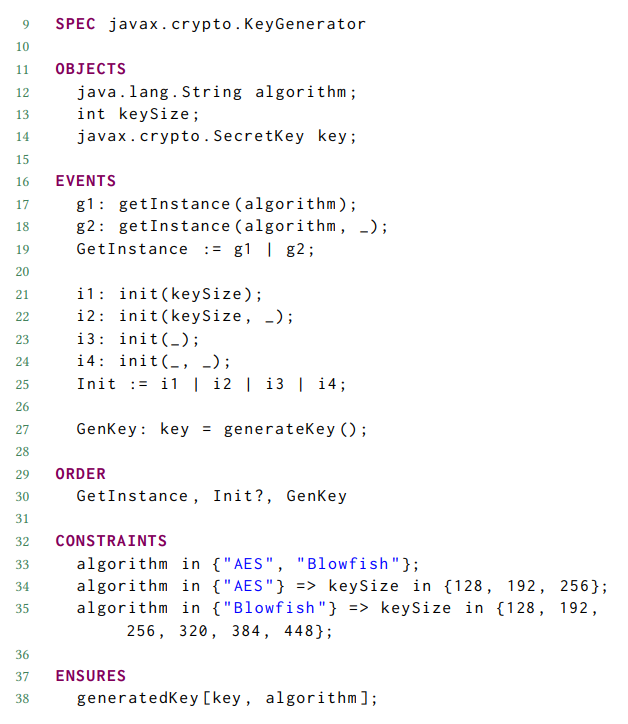
\includegraphics[width=0.7\textwidth]{CrySL}
\caption{CrySL Ruleset for JCA's \lstinline|KeyGenerator| class (Krüger \etal, 2017, \cite{kruger2017}, p. 3)}
\label{fig:CrySL}
\end{figure}
There are 6 mandatory sections for each CrySL file:
\begin{itemize}
	\item SPEC: the class to which the rules apply
	\item OBJECTS: the list of objects that will be used later in the rule set
	\item EVENTS: the list of methods that my contribute to the successful usage of the API. Similar methods (\ie  overloads) may be aggregated (\ie lines 17-19: the \lstinline|getInstance(...)| method is overloaded).
	\item ORDER: the order in which the events must be executed.
	\item CONSTRAINTS: accepted values for the specified object ("internal constraints"). We may also define dependencies (\ie lines 34 and 35: accepted key sizes depend on the algorithm) 
	\item ENSURES: predicates to govern interactions between different classes.
\end{itemize}
The CrySL definition language additionally allows to define illegal events in the FORBIDDEN section and kill existing predicates in the NEGATES section.\\

\par
Krüger \etal also implemented CogniCrypt, a compiler that translates CrySL rules into a static analysis which automatically checks a given Java application for rule violations \cite{kruger2017}.
To evaluate it, they defined  a rule set for JCA library and analyzed 10,001 Android apps and compared the results to the findings of a manual review of 50 randomly chosen apps.
They found at least one API misuse in 96 \% of apps that made use of JCA library.
CogniCrypt discovered 19,756 rule violations in 4,071 apps.
Most of them referred to broken constraints, especially for the \lstinline|MessageDigest| class.
When Kühne \etal found in their manual analysis that some programmers still used MD-5 and SHA-1 hash functions although these are considered broken.
CogniCrypt also identified a large number of misuses of the \lstinline|Cipher| class, especially the use of broken algorithms (DES) and unsafe encryption modes (ECB).
Another common misuse was that programmers forgot to clear the password at the end of the lifetime of a \lstinline|PBEKeySpec| object.\\

\par
Hazhirpasand \etal also used CogniCrypt to analyze 489 open source Java projects that made use of the JCA library \cite{hazhirpasand2020}.
Only 2 of them were considered as completely secure.
\begin{figure}[h]
\centering
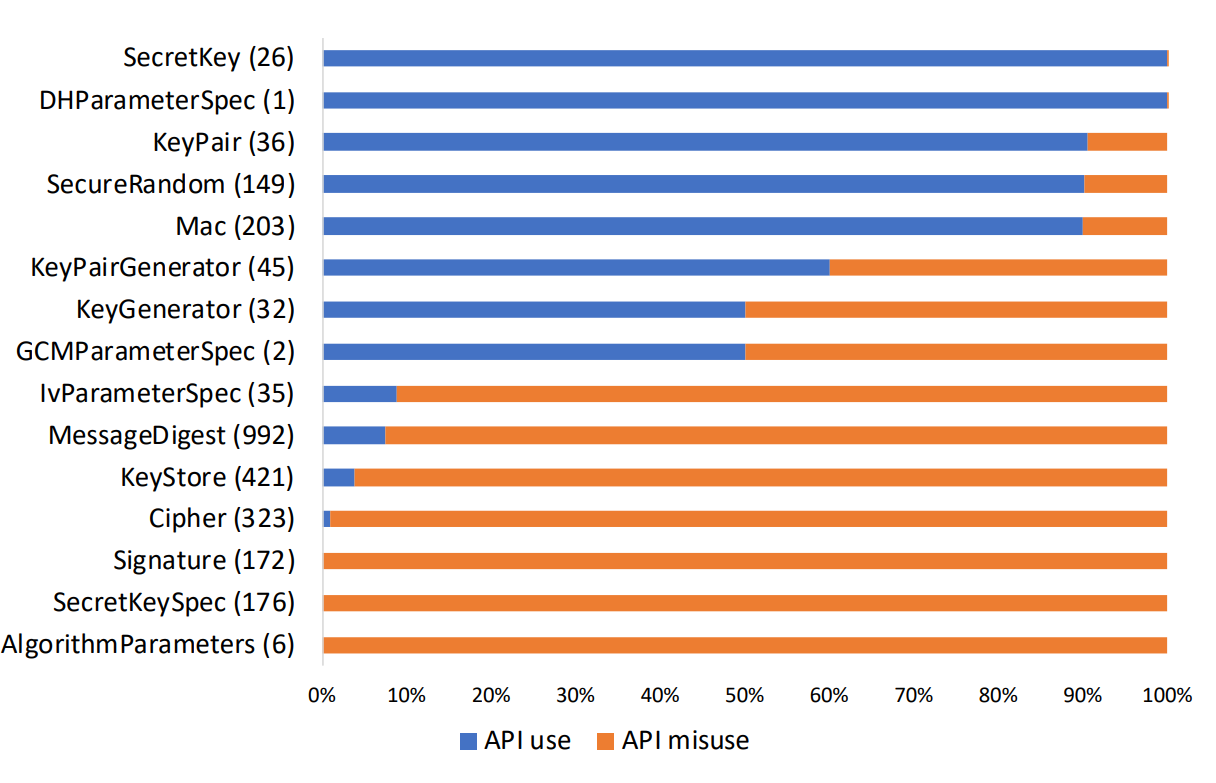
\includegraphics[width=0.9\textwidth]{APIMisuse}
\caption{Correct API use vs. API Misuse (Hazhirpasand \etal, 2020, \cite{hazhirpasand2020}, p. 3)}
\label{fig:APIMisuse}
\end{figure}
Figure \ref{fig:APIMisuse} shows the ratio of correct and incorrect usage for each of the investigated APIs.
Although a few records were mistakenly marked as misuse according to the authors manual review, their findings showed that programmers especially struggled to use the classes
\lstinline|AlgorithmParmeters|, \lstinline|SecretKeySpec|, \lstinline|Signature|, \lstinline|Cipher|,\lstinline|KeyStore|, \lstinline|MessageDigest|, and \lstinline|IVParameterSpec| correctly.
These classes are used to implement (symmetric) encryption, hashing, and digital signatures.\\
Hazhirpasand \etal also contacted 216 maintainers of the repositories to understand the reasons for API misuse.
Their answers implied that developers often underestimated the impact of cryptography misuse in publicly accessible code. 
They were not aware that 
and were not aware that their publicly accessible code could influence other programmers who were looking for examples. 
Some maintainers also lacked security knowledge.
They did not know how to use the API correctly and accepted security related pull request blindly.
Another identified issue was that there were not enough security concerns in the official documentation.
Sometimes, programmers also argued that although they use a cryptographic API, the code was not security related.\\

\newpage
\par
Piccolboni \etal also developed a tool to check security related code for API misuse: CRYLOGGER \cite{piccolboni2020}.
Unlike CogniCrypt, CRYLOGGER conducts the analysis dynamically by logging the parameters that are passed to the cryptography APIs during the execution. 
It later checks their legitimacy using a list of security related rules (see figure \ref{fig:CryloggerRules}).
\begin{figure}[h]
\centering
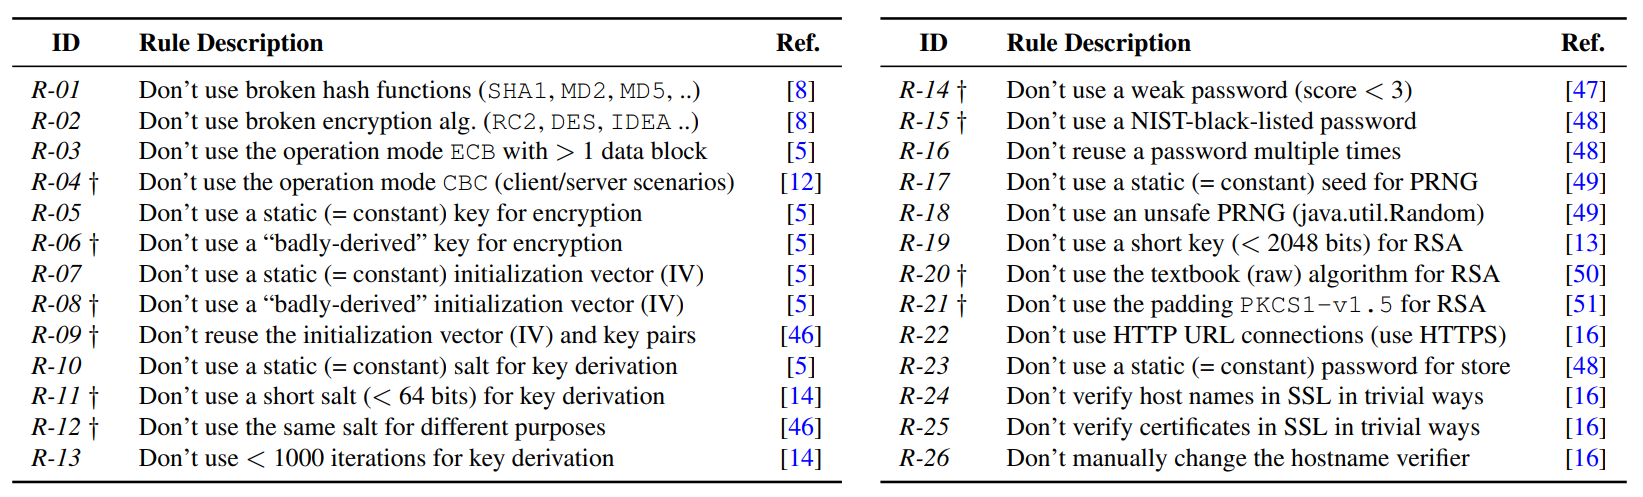
\includegraphics[width=1\textwidth]{CryloggerRules}
\caption{CRYLOGGER's Security Rules (Piccolboni \etal, 2020, \cite{piccolboni2020}, p. 5)}
\label{fig:CryloggerRules}
\end{figure}
Piccolboni \etal used CRYLOGGER to analyze 1,780 Android apps.
They found that rules 01 and 18 were violated very often ($> 90\%$).
This implied that broken hash functions and unsafe sources for random number generation were used very frequently.
They also found a rather high prevalence of violations for rules 04, 05, 06, 07, 09 and 22 ($> 30\%$) which refer to unsafe keys and initialization vectors, the reuse of key-IV pairs and the use of HTTP protocol.\\
\begin{figure}[h]
\centering
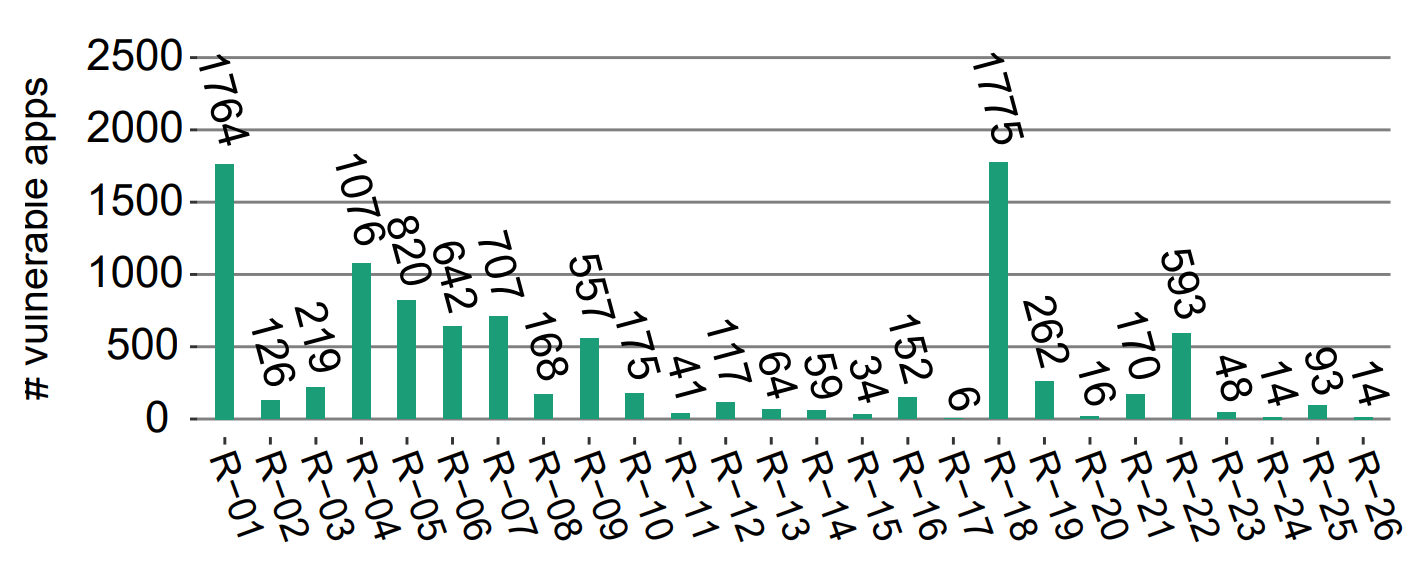
\includegraphics[width=0.7\textwidth]{RVPiccolboni}
\caption{Rule Violations Detected by CRYLOGGER ($N=1,780$) (Piccolboni \etal, 2020, \cite{piccolboni2020}, p. 12)}
\label{fig:CryloggerRules}
\end{figure}




% === M E T H O D O L O G Y ===
\chapter {Methodology}
\label{cha:Method}
To answer our research questions, we first had to identify the issues programmers face when implementing symmetric encryption using JCA.
We derived them by analyzing 150 threads on Stack Overflow which is one of the most popular Q\&A forums for programmers.
We also scanned those threads regarding security risks.
We then reprocessed the results to define a set of questions that should be answered in the documentation.
Finally, we checked the documentation to see whether those questions are answered or not.\\

\par
As we required several methodical approaches, this chapter is divided into five sections.
The first section describes the sampling process.
The second section refers to identifying issues from Stack Overflow posts.
The third section explains how we checked the threads for security issues.
The fourth and last section is about the analysis of the library's documentation.\\

\newpage
% === Sampling ===
\section{Sampling}
\label{cha:MetSampling}
In JCA, symmetric encryption is implemented using the \lstinline|Cipher| class.
It supports a wide range of symmetric and asymmetric encryption algorithms.
To search for suitable threads on Stack Overflow, we first defined a set of queries.
We use the \lstinline|[java]| tag combined with a minimal \lstinline|Cipher.getInstance()| statement for each symmetric algorithm.
This statement must be executed in all encryption scenarios using \lstinline|Cipher| class.\\
As some of the symmetric algorithms supported by JCA are not very popular, the corresponding queries returned only a small amount of posts.
We decided to exclude those algorithms and focused on the three most popular symmetric encryption algorithms: AES, DESede and DES.\\
\par
Next, we calculated the sampling size using the \href{https://www.surveymonkey.com/mp/sample-size-calculator/}{sample size calculator by SurveyMonkey}.
To ensure a confidence level of 95\% and a margin of error below 8\%, we required 150 posts.
Then, we computed sample size per query proportionally to the number of posts a it returns.
The result can be found in table \ref{tab:SampleSize}.

%=== Do Not Change This Table! ===
\begin{center}
\begin{table}[h]
% === Sampling Sizes JCA
\begin{tabular}{|m{8cm}|m{2cm}|m{3cm}|}
\hline
\textbf{Query} & \textbf{\#Posts} & \textbf{Sample Size} \\
\hline
\lstinline|[java] Cipher.getInstance(AES)|&3233&126\\
\hline
\lstinline|[java] Cipher.getInstance(DESede)|&295&12\\
\hline
\lstinline|[java]Cipher.getInstance(DES) --DESede|&300&12\\
\hline
\end{tabular}
\caption{Computation of Sample Sizes}
\label{tab:SampleSize}
\end{table}
\end{center}
%=======================================
\par
Finally, we selected the threads.
We picked half of the sample from the newest\footnote{based on the creation date of the question} threads and the other half from the most popular\footnote{based on the view count} ones.
This approach attempts to balance the ambition to detect present issues with the fact that most programmers first search for answers on Stack Overflow (generating views) before posting a question.\\
As the aim of the analysis was to reveal issues referring to the implementation of \emph{symmetric encryption} using the \emph{JCA} library, we excluded all posts that did not refer to this scope.
Of course it is possible that several issues are discussed in one thread.
A thread was included if at least one issue, question, or advise referred to our scope.

\newpage
% === Analysis 1 ===
\section{Analysis of Issues}
\label{cha:MetIssues}
The goal of the first analysis was to answer the first research question: \emph{What issues do programmers face when implementing symmetric encryption using Java Cryptography Architecture?}
We followed the guidelines for qualitative content analysis by Mayring \cite{mayring2015}. 
They are a standard in humanities to evaluate text-based data and are especially well suited for method-integrative approaches that combine qualitative and quantitative elements.
They allow to evaluate large amounts of material and quantify individual analysis steps - which is exactly what we need to answer our first research question.
They also provide a set of criteria to evaluate the validity and reliability of a methodical approach.\\
In this section, we will only provide the information to understand the process. You can find the complete processing scheme in the "Anleitung zu Wissenschaftlichen Arbeiten", chapter \ref{cha:AWI}.\\
\par
We conducted the analysis in three rounds.
We first applied \emph{summarizing} to extract the relevant information (issues and questions) from the threads.
Then we classified the issues in two rounds.\\

% === Summarizing ===
\subsection{Summarizing}
The goal of this first analysis step was to extract all relevant information and record it such that we did not have to re-read the entire threads during further evaluation.
We considered the question post, posts marked as "accepted answers" as well as comments to those posts.
If there was not any accepted answer, we considered all posts and comments and tried to display the discussion in our records.\\
We conducted summarizing first on our own and discussed the results afterwards to create a consistent and more objective list of records.
In particular, we eliminated records that did not refer to our scope.
As an example, we excluded all issues that referred to the conversion of plain text or the cipher text as data conversion (or character encoding) is not only required in the context of cryptography.
\par
For each thread, we recorded the set of issues and questions that the original poster\emph{author of the question post} was facing.
Then we tried to identify the reasons and solutions or answers.
We aimed for a short issue description (e.g. an error message or a shortened form of a question) and more precise explanations for the reasons and solutions.
To stay as near to the material as possible, we copy-pasted words, sentences or even paragraphs.\\

\newpage
% === Classification ===
\subsection{Classification}
As already mentioned, we classified the threads in two rounds regarding two different kind of aspects. 
We first classified all records regarding technical aspects and then classified the records regarding requirements the original poster was not able to meet.
In each round, we assigned at most one category to a record.
We also wanted to assign at least one category to each record.
So in the end, a record should have one or two assigned categories.

% Technical Aspects / Implementation
\subsubsection*{Technical Aspects}
In the first round of classification, we focused on the technical aspects of implementing symmetric encryption.
As categories, we defined a set of tasks that programmers must take care of when implementing symmetric encryption using JCA.
If they implement all tasks correctly, the code compiles and runs without rising an error and leads to the expected result.
So if programmers ask questions on Stack Overflow about a technical aspect, they either implemented a task incorrectly or they have a question regarding one of these tasks. 
In this classification we asked 
"What implementation step was performed incorrectly causing the error?" or 
"What implementation step is targeted by the question?".\\

Identifying a set of main tasks was simple: \emph{Cipher Object Instantiation, Generating Algorithm Parameters, Cipher Object Initialization, Transformation, and Transmitting Algorithm Parameters}.
But as we wanted to have more insight, we also defined subcategories.
To do so, we consulted the "Java Cryptography Architecture (JCA) Reference Guide" \cite{javaReferenceGuide} which provides code examples as well as explications regarding the use of the different APIs.
To allow an unambiguous category assignment, we also defined the dependencies as categories.
As a result, the following technical categories and subcategories were derived:
\begin{itemize}
	\item \textit{Cipher Object Instantiation}:
				We assigned this category to all issues and questions referring to an inappropriate \lstinline|Cipher.getInstance(...)| statement.
				As parameter, programmers must pass a transformation string consisting of:
				\begin{itemize}
					\item \textbf{Algorithm} (mandatory)
					\item \textbf{Encryption Mode} (optional)
					\item \textbf{Padding Mode} (optional)
				\end{itemize}
				Additionally, we defined the following subcategories:
				\begin{itemize}
					\item \textbf{Dependency Encryption Mode - Padding}: The encryption modes determines whether padding is required or not.
								We assigned this category to all issues caused by an inappropriate specification of those two properties.
					\item \textbf{Cipher Object Instantiation - Other} for issues and questions related to \lstinline|Cipher| object instantiation but not any of the aforementioned aspects.
				\end{itemize}
	\item \textit{Generating Algorithm Parameters}: 
				Depending on the specification of the cipher object, it requires different kind of parameters. 
				For encryption, the programmer might need to perform the following tasks:
				\begin{itemize}
					\item \textbf{Key Derivation} for issues and questions referring to random key generation, password based key derivation or key exchange protocols.
					\item \textbf{Initialization Vector / Nonce Generation} for issues and questions referring to the generation of the IV or nonce used for the transformation.
					\item \textbf{Generation of Other Algorithm Parameters}, e.g. a \lstinline|GCMParameterSpec| object which contains additional parameters for GCM encryption mode.
				\end{itemize}
	\item \textit{Cipher Object Initialization}: We assigned this category to all issues caused by the misuse of the \lstinline|init(...)| statement, e.g. not passing all required
						parameters. We defined the following subcategories:
				\begin{itemize}
					\item \textbf{Dependency Algorithm - Key}: The algorithm determines what data type the key must be stored in. 
									It also defines the allowed key sizes.
									We assigned this category to issues caused by passing an inappropriate key to the \lstinline|init(...)| method or questions about this dependency.
					\item \textbf{Dependency Algorithm \& Encryption Mode - IV}: The encryption mode determines, whether an IV is required or not.
									For some encryption modes (e.g. "CBC") the IV must be the same size as the algorithms block size.
									As an example, an issue related to passing an IV of the wrong size to the \lstinline|init(...)| method was assigned to this category.
					\item \textbf{Cipher Object Initialization - Other}
				\end{itemize}
	\item \textit{\textbf{Transformation}}: This category was assigned to all issues and questions targeting the actual transformation methods \lstinline|update(...)| and \lstinline|doFinal(...)|, e.g. passing the wrong input parameters or questions about the output.
	\item \textit{Transmission of Parameters}:
				As all parameters from encryption must be reused for decryption, they must either be stored or transmitted. 
				This category was assigned to all issues and questions referring to storing, restoring, or transmitting parameters.
				We defined the following subcategories:
				\begin{itemize}
					\item \textbf{Key Transmission}: The key must be kept secret.
					\item \textbf{Transmission of Other Parameters} such as the initialization vector. 
						They can be transmitted along the cipher text as they do not have to remain secret.
	 			\end{itemize}
	\item \textbf{Dependency Encryptor - Decryptor}: 
				The \lstinline|Cipher| objects used for encryption and decryption must be specified and initiated in the exact same way except for the parameter specifying the operation in the \lstinline|init(...)| statement.
				We assigned this category to all issues caused by differing configurations.
\end{itemize}
You can find a list with concrete examples for each category in the appendix.\\ %ToDo

\begin{figure}[h]
\centering
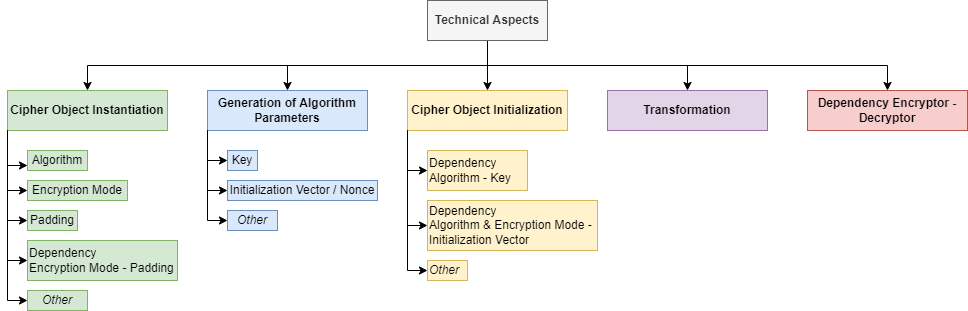
\includegraphics[width=1\textwidth]{Categories}
\caption{Hierarchy of Technical Aspects Categories}
\label{fig:Categories}
\end{figure}


% Implications / Requirements
\subsubsection*{Requirements}
As the first set of categories only targeted the implementation of symmetric encryption, we defined a second set of categories regarding the design of an application.
We defined different kind of functional and non-functional requirements as categories.
We consulted  Sommerville \cite{sommerville2011} as a theoretical basis.
During the analysis we asked ourselves "Which requirements are not met?".
Not all requirements defined by Sommerville occurred in our analysis.
We only assigned the following categories:
\begin{itemize}
	\item \textbf{Functional Requirements} to issues where a programmer was not able to fulfill a certain requirement or tried to use encryption for an unsuitable use case.
	\item \textbf{Performance} to issues where an implementation was not as time-efficient as required.
	\item \textbf{Space} to code leading to an \lstinline|OutOfMemoryException|.
	\item \textbf{Reliability} to situations where the implementation crashed frequently.
	\item \textbf{Portability} to implementations that behaved differently on different (Java) plattforms.
	\item \textbf{Interoperability} to issues where a developer was not able to decrypt a cipher text that was produced using another library or vice versa.
	\item \textbf{Security} to implementations containing security risks.
\end{itemize}
\par
As we analyzed the discussion, we only assigned a category if either the original poster complained about not being able to meet a certain requirement or someone gave a hint.
We conducted a broader examination of security risks in our second analysis (see chapter \ref{cha:MetSec}). 


% Evaluation
\subsection{Evaluation} % ToDo
We conducted several forms of frequency analysis' on our data.
We computed the absolute and relative frequencies for each category and subcategory.
Finally, we also took a look at the combination of technical aspects and requirements categories.
In our interpretation, we focused on the most occurring categories as these refer to more prevalent issues.\\
\colorbox{yellow}{ToDo}

% === Analysis 2 ===
\section{Analysis of Security Risks}
\label{cha:MetSec}
The goal of this second analysis was to answer the second research question: 
\emph{What are common security risks in code and advises shared on Stack Overflow referring to the implementation of symmetric encryption scenarios Java Cryptography Architecture?}\\
We first defined a set of security rules regarding the implementation of symmetric encryption.
Then we reprocessed the original sample checking them for rule violations.

\subsection{Security Rules}
We derived our rules from the rule sets used for CRYLOGGER tool (see Piccolboni \etal \cite{piccolboni2020}) and the CrySL based compiler for Java applications by Krüger \etal \cite{kruger2019}.
We only considered the rules that were applicable to symmetric encryption and structured them using the categories from technical aspect's classification (see section \ref{cha:MetIssues}).
We also abstracted the context of the rules to facilitate their evaluation.
As an example, R-04 of CRYLOGGER says " Don’t use the operation mode CBC (client/server scenarios)" (Piccolboni \etal, 2020, \cite{piccolboni2020}, p.5).
We abstracted the context and defined that a programmer should not use CBC at all.
We often do not know in what context the original poster wanted to use the code.
Additionally, if we think about someone naively copy-pasting code from Stack Overflow, the use of CBC is a potential security risk.\\
The resulting rules can be found in table \ref{tab:Rules},

\subsection{Tracking Security Rule Violations}
We reprocessed the original sample marking for each rule whether it was violated or not.
We only considered the question post, the accepted answer post, and comments to one of these.
We also distinguished between "question" and "answer" as well as "code" and "text".
We analyzed the four aspects independently and made a list for each one of them:
\begin{itemize}
	\item \textbf{Question Code} to track security risks in code snippets of the question post
 	\item \textbf{Question Text} to track security risks in the text of the question post as well as comments to it by the original poster
	\item \textbf{Answer Code} to track security risks in code snippets of the answer post
	\item \textbf{Answer Text} to track security risks in the text of the answer post as well as any comment by another person.
\end{itemize}
While analyzing the code snippets, we focused on the parts where encryption, decryption, key derivation, IV generation, and key storage were implemented.
As an example, if someone is defining a static key in the main method and passes it to the encryption section as a parameter, we did not consider this a security risk.
The encryption section can still be safe if an appropriately derived key is passed.\\
The answers were only analyzed if there was an accepted one.\\
\begin{table}[h]
\centering
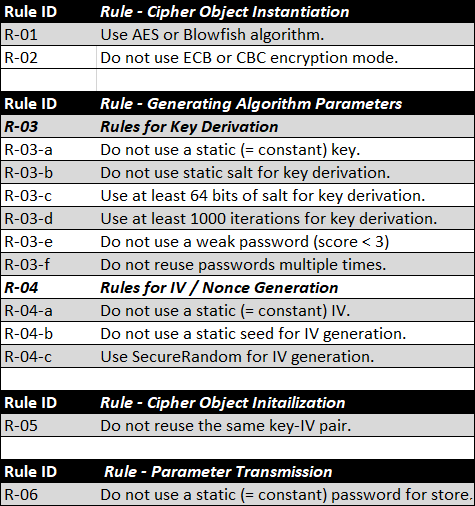
\includegraphics[width=0.7\textwidth]{Rules}
\caption{Security Rules}
\label{tab:Rules}
\end{table}

\subsection{Evaluation}
We conducted a frequency analysis for each list.
Our aim was to find out the most prevalent security risks to answer the research question. \colorbox{yellow}{ToDo}\\


% === Analysis 3: Documentation ===
\section{Analysis of Documentation}
\label{cha:MetDoc}
The results from the precedent analyses formed the basis to analyze the documentation for JCA.
As it spreads over several documents and sources, we only examined the most basic ones:
the Java Cryptography Architecture (JCA) Reference Guide \cite{javaReferenceGuide}, 
the Java Security Standard Algorithm Name Specification \cite{javaStandardAlgorithmName}, 
and the entire API documentation for \lstinline|javax.crypto| package starting from the package overview \cite{javaxCrypto}.
These three documents are valid for all providers and therefore apply to a wide range of platforms.\\
\par
To analyze the documentation, we first defined a set of question that should be answered.
Afterwards, we sought the answers in the documentation.
Our aim was to answer the third research question: 
\emph{To what extent are those issues\footnote{obstacles in implementation, security risks in code} linked to missing or inadequate documentation?}
The questions additionally gave us more insight in what programmers are struggling with.
They helped us to answer then first research question more precisely.

\subsection{Deriving Questions}
As an API documentation should support the usage of the API and not educate the programmer, basic questions regarding cryptography should not be answered in it.
However, a cryptography API should link reliable sources (\ie Mindermann \etal \cite{mindermann2018}).
We therefore created two lists of prioritized questions: one with "questions to documentation" and one containing "general questions".\\
\par
We derived the questions from the results of the former analyses.
We reprocessed the records from the first analysis and tried to formulate a question for each one.
If the question was new, we wrote it down and set its priority to one.
If there was already a similar question, we increased its priority by one and sometimes reformulated the question.\\
The set of questions derived from the first analysis' results covered already a wide range of security related topics.
We therefore did not have to add more questions based on the second analysis' findings.
However, we adapted the priorities of those questions, setting them to the actual number of threads that included a related security risk.

\subsection{Consulting Documentation}
For each question on the list, we then tried to find an answer in the documentation.
Depending on the question, we checked the different sources in another order.
We aimed to find answers as efficiently as possible.\\
For "questions to documentation", we typically started with the reference guide to find general explanations and then consulted the related parts of the API documentation.
For "general questions" we started in the standard algorithm name specification.
Of course, we knew the documentation better after answering a set of questions and therefore optimized our search strategies.\\
Once we found an answer to the question, we recorded its source as well as some remarks regarding documentation quality.

% === Evaluation ===
\subsection{Evaluation}
We first wanted to find out, what percentage of questions remained unanswered.
This gave us a starting point to answer the research question.
If most questions are answered in a clear way, we cannot blame the documentation for the issues programmers face during implementation.
We also cannot blame it for unsafe code if it contains enough hints and advises regarding security.\\
In the further evaluation we focused on the unanswered questions and our comments regarding documentation quality to make suggestions regarding the improvement of the documentation.\\
We also had a closer look at the questions as they gave us more insight regarding the first research question.\\



% === R E S U L T S ===
\chapter {Results and Interpretations}
\label{cha:Results}
In this chapter, we discuss the results of our three analyses and their interpretation.
There is a section for each of the three conducted analyses:
The first section presents the issues programmers faced during the implementation of a symmetric encryption scenario using JCA library.
The second section discusses the security risks we found in our sample data.
The third section explains how the previous findings are linked to the documentation.\\


% === Issues ===
\section{Implementation Issues}
\label{cha:ResIss}
In our first analysis, we tried to identify all issues the original posters were facing and recorded them separately.
Depending on what the original poster was struggling with, we afterwards classified the issues as relating to a \emph{technical aspect} and/or a \emph{requirement}.\\
In total, we recorded 219 issues.
We classified 197 (90\%) of these records regarding technical aspects and 76 (35\%) regarding requirements. 
62 records were classified twice.
We could not classify only one thread (and its relating record) to the lack of adequate information.\\
\begin{figure}[h]
\centering
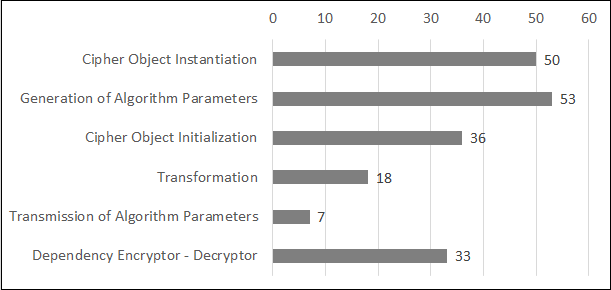
\includegraphics[width=0.85\textwidth]{TechnicalAspects}
\caption{Number of Issues Assigned to a Technical Aspects Main Category ($N = 219$)}
\label{fig:TechAspPlot}
\end{figure}

\par
% === Technical Aspects ===
As shown in figure \ref{fig:TechAspPlot}, the most common categories in the first round of categorization were \emph{Generation of Algorithm Parameters} (50) and \emph{Cipher Object Instantiation} (53). 
Both of these categories refer to specifying and generating the properties that are used during encryption or decryption.
During the generation of algorithm parameters, programmers might derive a key, an initialization vector, and other algorithm parameters such as advanced authentication data.
The original posters especially struggled with key derivation (36 records - 16.4\%).
This was not surprising as previous work has already revealed that programmers struggled with key handling.
The set of issues referring to the key\footnote{derivation, transmission, dependency from algorithm} made up more than $\frac{1}{5}$ of all issues.\\
During the instantiation of a \lstinline|Cipher| object, programmers specify the algorithm, the encryption mode, and padding.
The original posters were especially struggling with the latter two.
18 records referred to the encryption mode, 11 to padding and another 11 to the dependency of these properties\\
\par
The third most common category was \emph{Cipher Object Initialization} (36). 
In this implementation step, the generated parameters (\ie key, IV,...) are passed to the cipher object.
Most issues were assigned to the \emph{other} subcategory.
They often refer to the default behavior of the \lstinline|init(...)| method if not all required properties were passed.\\
\par
The fourth most common category was \emph{Dependency Encryptor - Decryptor} (33).
More than 27\% of all issues referred to a dependency related subcategory.
The high prevalence of issues referring to the dependency of encryptor and decryptor implies that people lack knowledge about (symmetric) encryption in general.\\
The fact that the cipher objects for encryption and decryption must use the exact same algorithms and parameters is \emph{the} basic principle of symmetric encryption.\\

\par
The other main categories and subcategories were not assigned that often.
Some original posters were confused that there were 2 methods that perform \emph{Transformation}: \lstinline|update(...)| and \lstinline|doFinal(...)|.
They did not know when which method must be called.
Also the output of encryption / input to decryption caused some issues when programmers used message authentication.\\
Among issues referring to the \emph{Transmission of Algorithm Parameters} (7), most referred to the key (5).
The remaining referred to the initialization vector (1) and to salt used during key derivation (1).\\
\par
You can find the complete list of subcategories and their frequencies of assignment in table \ref{tab:TechAspTab}.\\
\begin{table}[h]
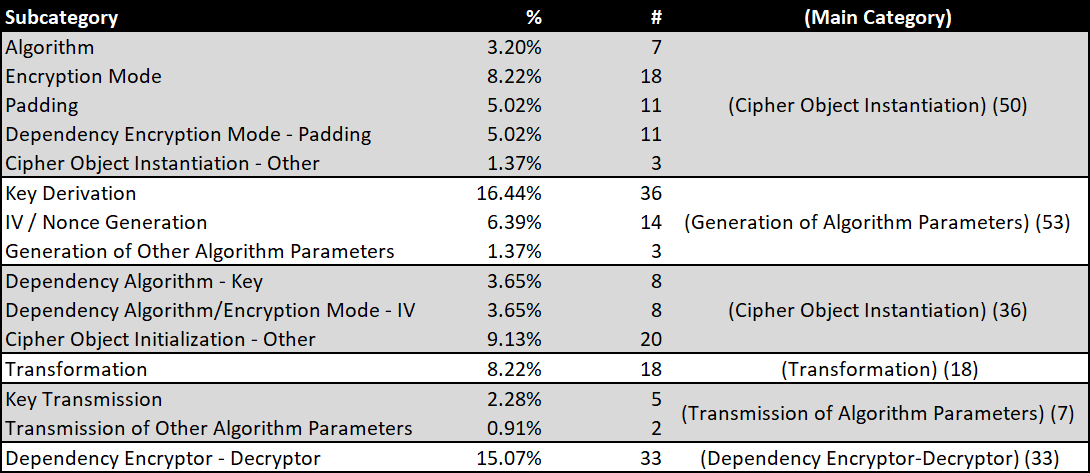
\includegraphics[width=1\textwidth]{TechAspTable}
\caption{Number of Issues Assigned to a Technical Aspect Subcategory ($N = 219$)}
\label{tab:TechAspTab}
\end{table}

% === Requirements ===
\par
Within the categories referring to requirements, \emph{Security} was the dominating category (46 records - 21\%).
This seems natural as this is what cryptography is all about.
However, most security issues were not mentioned in the question post.
They refer to security hints by people commenting or answering. 
Yet, there is massive under-reporting as our results from the security related analysis show (see section \ref{cha:ResSec}).\\
The other categories occurred much less often as you can see in figure \ref{fig:Req}
\begin{figure}[h]
\centering
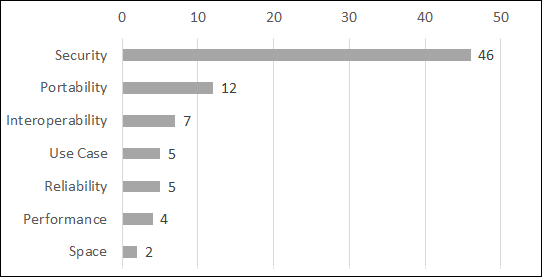
\includegraphics[width=0.8\textwidth]{Requirements}
\caption{Number of Issues Assigned to a Requirement Category ($N = 219$)}
\label{fig:Req}
\end{figure}

\newpage
\par
% === Doubly Classified Records ===
We observed the highest overlapping of categories for \emph{Generation of Algorithm Parameters} and \emph{Security} as well as 
\emph{Cipher Object Instantiation} and \emph{Security}. The heat map in figure \ref{fig:HeatMap} shows the relative overlapping of categories:
21\% of all posts classified as \emph{Generation of Algorithm Parameters} or \emph{Security} issue were assigned to both categories.
As we had less data for the other requirements categories, it is not surprising that we found much less overlapping for those.\\
\begin{figure}[h]
\centering
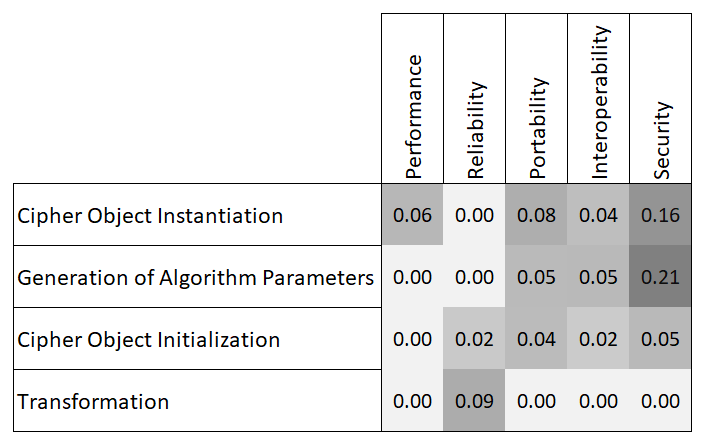
\includegraphics[width=0.8\textwidth]{HeatMap}
\caption{Relative Overlapping of Technical Aspects and Requirements Categories}
\label{fig:HeatMap}
\end{figure}



\newpage
% === Security ===
\section{Security Risks}
\label{cha:ResSec}
We manually checked 150 question,  84 answer posts, and related comments using our rule set.
We found a total of 331 security risks.
Most of them (249 - 75\%) stem from code snippets in question posts.
The text of question posts included only 38 security risks.
But we observed that the questions often did not contain much text.\\
We found 35 rule violations in answer related code snippets and 9 in related text.
We observed that some answers just fixed the functionality of a question related code section without improving its security.
The resulting code therefore "inherited" the security risks from the question.
Another common observation was that people correctly gave the hint that ECB was not considered safe.
However, they suggested to use CBC instead which must not be used in client-server scenarios.
Such advise is therefore not safe, especially if we do not know in what kind of application the code section is used.\\
\begin{table}[h]
\centering
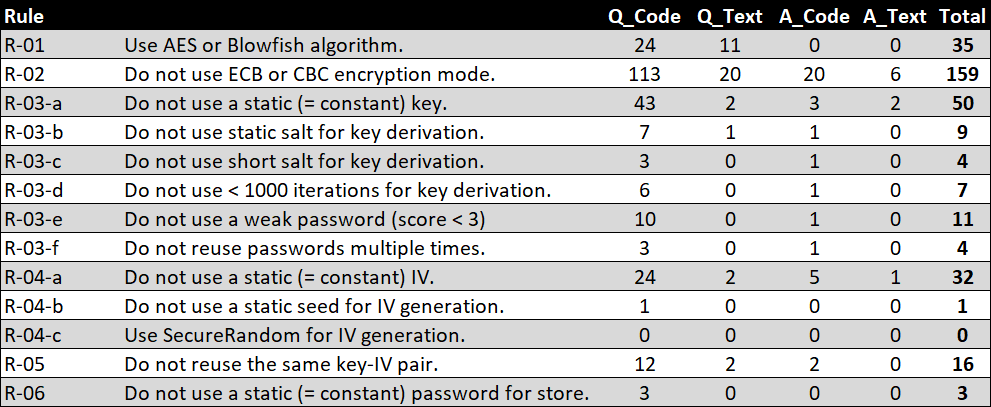
\includegraphics[width=1\textwidth]{SecTab}
\caption{Rule Violations per Check List}
\label{tab:SecRisk}
\end{table}
\par
% === Question Related Code
As we found code snippets in all question posts and therefore have most data for them, we focused on the evaluation of that check list.
The average question post contained 1.66 security risks in its code snippets.
We observed that the average for the most popular (and older) posts (1.91) is slightly higher than the one for the newest posts (1.43).
24 question posts did not contain any security risk in their code snippets.\\
The most often violated rule was \emph{R-02: Do not use ECB or CBC encryption mode}. 
In more than 75\% of question posts, the original poster used one of these unsafe block cipher modes.
This is also due to ECB being the default encryption mode.
It is followed by the presence of constant keys (\emph{R-03-a}), unsafe password based key derivation procedures (\emph{R-03-b to R-03-f}, 29 recorded rule violations), and static
initialization vectors (\emph{R-04-a}).\\
Of course, the number of posts showing violations of \emph{R-01} is strictly related to the sample: 24 of our threads referred to DES or TripleDES encryption.
There were some code snippets in which the same key-IV pair was reused for several encryption operations.
This was related to using a constant key and a constant IV in most cases.


% === Documentation ===
\section{Documentation}
\label{cha:ResDoc}
We derived a total of 64 questions: 43 referring to documentation and 21 more general ones.
After checking the documentation, 10 questions remained unanswered and for 15 questions, we considered the answer as incomplete, unclear, or even misleading.\\

\subsection{Questions}
Our first observation regarding the questions was that there are twice as many JCA-specific questions as general ones.
Yet, the total priority of all "general" questions was much higher than the total priority of the specific ones even before correcting the priority for the security relevant ones.
This indicates one more time that programmers asking questions on Stack Overflow do not only lack knowledge about the JCA library but also about cryptography in general.\\

\par
The results from the first analysis gave us insight in what tasks and requirements programmers are struggling with.
The questions helped us to detect API related issues.
8 questions targeted a specific platform or were related to providers. 
2 of them were among the 3 most prioritized questions to documentation. 
As an example, the default behavior of a \lstinline|Cipher| object if not all required properties were specified during object instantiation or initialization also depends on the provider.
However, whether a provider is available or not and which provider is used by default depends on the platform.\\
Another 5 questions were related to method overloads. 

There are two methods that perform the data transformation and both of them are overloaded.
The methods for instantiation and initialization are overloaded as well.
\begin{table}[h]
\centering
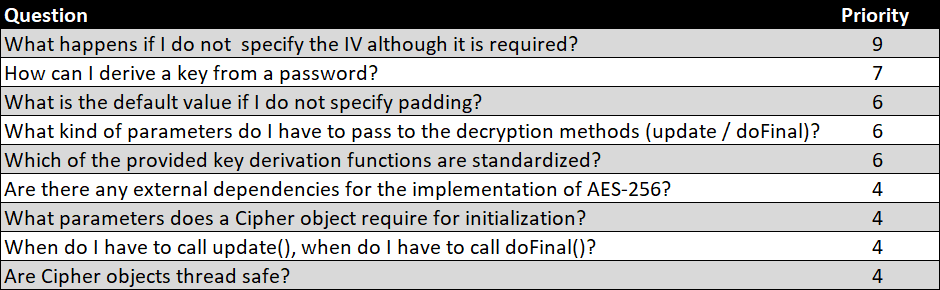
\includegraphics[width=1\textwidth]{QuestionsToDoc}
\caption{Top 9 JCA-Specific Questions}
\label{tab:Ques}
\end{table}

\subsection{Missing and Unclear Answers}
We were not able to find and answer to 3 JCA-specific and 7 general questions.
They all had a rather low priority (< 4).
The higher prevalence of unanswered general questions implies that JCA documentation does not provide (enough) links to trusted resources for general information about cryptography.\\
The following three unanswered questions represent documentation related issues:\\
\begin{itemize}
	\item \emph{How to specify PKCS\#7 padding in Java?}
					PKCS\#7 is a standardized padding for arbitrary block sizes that is supported by many cryptography libraries.
					JCA internally interprets PKCS\#5 padding as PKCS\#7 if it is required.
					However, this is not mentioned in the Standard Algorithm Name Specification nor in any other document that we examined.
					This might complicate the implementation of interoperability scenarios.
	\item \emph{What properties does AES-256 require?}
					There is a link to the official specifications for most algorithms in the Standard Algorithm Name Specification.
					However, for AES there is not.
					This is problematic since AES is one of only two symmetric encryption algorithms that are recommended.
	\item \emph{Which symmetric encryption algorithms are safe to use?}
					JCA documentation does not provide enough hints regarding security. 
\end{itemize}

\par
For 13 JCA specific questions and 2 more general ones, we considered the answers as not clear enough.
They often referred to method overloads. 
The documentation did not point out the differences clearly enough.
It often seemed like copy pasted.\\
Another common issue was that there is not any code example for some key scenarios (e.g using a \lstinline|KeyStore| or password based key derivation using PBKDF2).
The available ones often did not work due to some missing parts:
The code example for encryption did not show how the algorithm parameters were generated.



% === D I S C U S S I O N ===
\chapter {Conclusion and Future Work}
\label{cha:Conclusion}
In this chapter, we first aim to answer our research questions based on our finding from the previous chapter.
We then discuss possible limitations of our study and suggest further research topics.
We finally draw a conclusion where we .
\colorbox{yellow}{ToDo}\\

\par{RQ 1}: \emph{What issues do programmers face when implementing symmetric encryption using Java Cryptography Architecture?}
Our study provided answers to this question from different perspectives:\\
If we think of \emph{tasks} that programmers are struggling with, most of them were struggling with key derivation and cipher object instantiation (especially specifying encryption mode and padding correctly).\\
The dependency from providers, unsafe default values, the existence of two kind of methods performing transformation, and the high amount of overloaded methods were the most common issues related to the \emph{library's design}.\\
But also the \emph{documentation} provided some obstacles.
It lacked working code examples, method overloads were documented too similarly, and there were not enough links to trusted sources for more general information about cryptography.\\
When we think of the \emph{programmers}, our study added more evidence confirming the assumption that they lacked knowledge about cryptography.
However, we would like to extend it:
As the scope of our study was quiet limited, we excluded all threads that did not target it.
To collect our sample, we had to exclude 296 threads.
For each thread that (partly) belonged to our scope, there were two threads that did not.
Of those excluded threads, 138 (ca. 47\%) did either not refer to cryptography at all or they did not refer to the JCA library.
The large amount of threads containing non-JCA-related issues let us conclude that programmers do also lack knowledge about computer science in general.
We therefore should be aware that cryptography scenarios are implemented by programmers of all kind of backgrounds when we design a cryptography library.\\

\par{RQ 2}: \emph{What are common security risks in code and advises shared on Stack Overflow referring to the implementation of symmetric encryption scenarios using JCA library?}
The most common security risk was the use of an unsafe encryption mode.
This is also related to JCA using ECB as default block cipher mode of operation.\\
Other common security risks were the use of static values for either key, initialization vector, or both.
Although some people explicitly stated that they only use them in their post on Stack Overflow to simplify the code section, it will become a security risk if we think of a programmer without knowledge about cryptography / software security naively copy-pasting the code.
The procedures used for password based key derivation also contained security risks.\\
We however observed a slight improvement when we compared the older posts with the newer ones.\\

\par{RQ 3}: \emph{To what extent are those issues linked to missing or inadequate documentation?}
This research question is the most difficult one to answer.
Most questions (>60\%) were clearly answered in the documentation, especially the higher prioritized ones.
We found related information for almost 85\%.
We therefore cannot blame insufficient documentation for the struggles of developers.
There are at least two other explanations:
Either, the programmers who asked those questions did not consult the documentation at all or they did not have enough knowledge to understand it.\\
Yet, the documentation could be improved.
It should provide more (working) code examples, security hints, and links to trusted resources for more information about cryptography.
In the API documentation, the method overloads should be documented more specifically.

\section{Limitations and Future Work}
As this project followed a qualitative approach and performed an in-depth analysis, it is reasonable to have a limited scope.
Future work must extend it by examining more use cases and libraries.\\

\par
When it comes to the methodical approach, one threat to validity is that the population of Stack Overflow threads matching our scope cannot be described exactly.
There is no guarantee that the used queries returned all posts referring to our scope.
Additionally, we had to exclude almost $\frac{2}{3}$ of all threads as they did not refer to our scope.
The sample can therefore not be considered as representative for the threads referring to our scope nor for the threads returned by our queries.
This implies that the results must be verified with further investigations.\\
Also, we did not verify the intercoder reliability of our issue classification or our security check.
It requires a certain expertise in cryptography and software security as well as experience with JCA library.
Our data is however published on GitHub\footnote{\colorbox{yellow}{ToDo}} and reanalyses are welcome.

\section{Conclusion}
Our study added more evidence confirming the findings of previous research.
Working with a low-level library such as JCA requires expertise.
Not all programmers working on security related code however have the required domain knowledge.



% === Future Work ===
% Findings from research must also be taken into account in the development of new libraries or in the refactoring of existing ones
% IT Industry must be aware of security and the need for expertise




% === A N L E I T U N G   Z U   W I S S E N S C H A F T L I C H E M   A R B E I T E N
\chapter {Anleitung zu wissenschaftlichen Arbeiten}
\label{cha:AWI}
This chapter describes the methodical approach of qualitative content analysis according Mayring \cite{mayring2015}.
Each section refers to a work step of the processing scheme which is first explained generally and then applied to the derivation of issues from Stack Overflow threads, see chapter \ref{cha:MetIssues}.\\
Please note that the aim of this chapter is to specify the processing scheme more precisely.
All kind of justification can be found in the methodology section of this thesis.

%ToDo: Citations?
\section{Presenting the Sample}
Defining and presenting the sample is the first step in qualitative content analysis: 
We describe the population, the context of its creation and its formal characteristics as well as the sampling process.

\subsection{Population}
Stack Overflow is one of the most popular online forums for programmers.
According to the developer survey from 2020, about 50 million people visit the platform per month.
Approximately 50\% of them are either professional developers or university-level students \cite{stackoverflow2020}.
As we only want to examine threads that refer to the implementation of symmetric encryption using the Java Cryptography Architecture library,
we define our population as the set of posts returned by at least one of the following queries:
\newpage
\begin{itemize}
	\item \lstinline|[java] Cipher.getInstance("AES")|
	\item \lstinline|[java] Cipher.getInstance("DESede")|
	\item \lstinline|[java] Cipher.getInstance("DES") --DESede|
\end{itemize}
\par
We do not know a lot about the context of our population.
Especially, we do not know anything about the people writing the posts and comments.
Based on the findings by Nadi \etal \cite{nadi2016}, we assume that the people asking questions are professional developers (industrial or freelance), researchers or students who must implement a symmetric encryption scenario either for work or education.
However, their backgrounds regarding experience with Java as a programming language or cryptography are very heterogeneous.
In Nadi \etal's survey, the test persons declared that they "spend at least several hours reading through online resources" (2016, \cite{nadi2016}, p. 938) before asking on Stack Overflow.\\
\par
All material is available online on Stack Overflow.
It reflects a conversation between one or several users.
For each post, we can see the username of the author as well as the date and time of its creation.
Some posts have been edited after their creation.
In that case, we can see the username and the date of the last edit.
However, we cannot reproduce what has been changed.
Sometimes, persons also delete their posts or comments.
Such posts are not visible anymore.


\subsection{Sampling Process}
Based on the total number of posts returned by the queries (3828) we calculated that 150 threads should be enough to satisfy our requirements of a confidence level of at least 95 \% and a margin of error below 10\%.
Next, we computed the number of threads per query proportionally to the number of posts it returned.
Finally, we selected the threads for our sample.
We picked half of the sample from the "newest" threads which was determined by the creation date of the question post.
We took the other half from the most popular ones based on the view count of the question.
Also, we only selected threads that addressed at least one issue within our scope.
Other posts were excluded for at least one of the following reasons: \colorbox{yellow}{ToDo: C\# Beispiele austauschen}
\begin{itemize}
	\item \textbf{too general}: posts referring to cryptographic concepts or cyber security in general rather than the targeted API\\ 
			\emph{Example: \href{https://stackoverflow.com/questions/939040/when-will-c-sharp-aes-algorithm-be-fips-compliant}{When will C\# AES algorithm be FIPS compliant?}}

	\item \textbf{does not refer to cryptography}: issues occurring in a non-cryptographic context, i.e. establishing a network connection or file access\\
			\emph{Example: \href{https://stackoverflow.com/questions/1755259/syntax-error-on-token-expected-after-this-token}{Syntax error}}

	\item \textbf{does not refer to symmetric encryption}: posts referring to other cryptographic concepts such as asymmetric encryption or hashing\\
			\emph{Example: \href{https://stackoverflow.com/questions/66941359/rsa-decryption-fails}{RSA decryption (fails)}} 

	\item \textbf{does not refer to JCA}: issues occurring during a symmetric encryption scenario but which are not due to Java Cryptography Architecture.
				Such issues can refer to another library (e.g. BouncyCastle) or to some other aspect such as character encoding.\\
				\emph{Example: \href{https://stackoverflow.com/questions/5641326/256bit-aes-cbc-pkcs5padding-with-bouncy-castle}{256bit AES/CBC/PKCS5Padding with Bouncy Castle}}

	\item \textbf{does not refer to targeted algorithm}: posts referring to other algorithms than the targeted ones\\
			\emph{Example: \href{https://stackoverflow.com/questions/68772573/how-to-use-password-with-pbekeyspec-hash}{how to use password with \lstinline|PBEKeySpec| hash}}

	\item \textbf{looking for an equivalent} or \textbf{interoperability issue}:  looking for equivalents / counterparts in different programming languages\\
			\emph{Example: \href{https://stackoverflow.com/questions/64902430/change-rijndael-decryption-logic-from-c-sharp-to-python}{Change Rijndael decryption logic from C\# to Python}} 

	\item \textbf{negative votes} or \textbf{closed}: posts of poor quality

	\item \textbf{academic}: posts with a different focus than obstacles when using the API

	\item \textbf{duplicate}: Duplicates are often left unanswered (or only answered with the reference to a similar post). For posts belonging to the "most popular" category, we included a duplicate if it had more views than the original.
\end{itemize}


\newpage
\section{Specific Research Questions}
The second step of qualitative content analysis is to describe precisely what the aim of the interpretation is.
We must provide a set of well defined research questions that are theoretically differentiated.\\

\par
The aim of our first analysis was to find an answer to the first research question of the thesis:
\emph{What issues do programmers face when implementing symmetric encryption using Java Cryptography Architecture?}
This question can be answered from several perspective.\\
As we wanted to analyze posts from Stack Overflow and people typically ask a question there if their code does not compile, throws a run-time error, or shows some other unexpected behavior, we first had a look at the \emph{technical aspects}.
When implementing  a symmetric encryption scenario, developers must take care of some properties (\ie algorithm, encryption mode, padding mode, key) and perform some actions with them (\ie derivation, storage, transmission).
Additionally, some of these properties depend on each other (\ie encryption mode - padding) (\ie see Nakov \cite{nakov2018}).
If any of these properties, actions, and dependencies is not implemented correctly, the code does not run or shows some strange behavior (\ie see JCA's Reference Guide \cite{javaReferenceGuide})\\
Once a system runs, it must meet various \emph{requirements}.
Sommerville distinguished between functional- and non functional requirements \cite{sommerville2011}.
He described functional requirements as a description of a system's the behavior and the services it provides (what a system should do).
He considered them as dependent from the type of software, the expected users, and the general approach of an organization when writing requirements.
He therefore did not define any sub-requirements.
Sommerville defined non-functional requirements  as constraints on the services and functions of a system (\ie memory limitations, time resources for development, legislative requirements).
As they are independent from the system, he presented a wide range of non-functional requirements (see figure \ref{fig:NonFuReq}).
\begin{figure}[h]
\centering
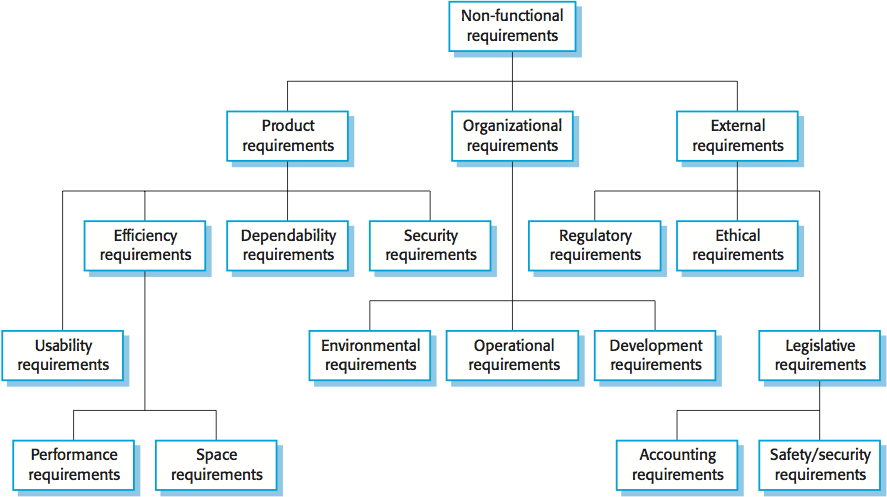
\includegraphics[width=0.8\textwidth]{NonFuReq}
\caption{Non-Functional-Requirements as defined by Sommerville (2011, \cite{sommerville2011}, p.88)}
\label{fig:NonFuReq}
\end{figure}

As we aimed to cover both perspectives with our analysis, we formulated the following specific research questions regarding the implementation of symmetric encryption scenarios using JCA library:
 \begin{itemize}
	\item What technical aspects do programmers fail to implement correctly?
	\item What requirements do programmers struggle to meet?
\end{itemize}

The categories that we used can

\section{Processing Scheme for Interpretation}
Summarizing:
The coding unit of this first round of analysis was a single word (e.g. an error message).
The context unit was an entire post or a comment.\\


\section{Evaluation of Specific Quality Criteria}

%ToDo: Kommt in "Anleitung zu wissenschaftlichem Arbeiten"
%To verify intercoder reliabilty, 15 posts per library (10\%) were randomly chosen and reviewed by two colleagues who were not involved in the project.
%After a quick introduction to the categories and the procedure, they followed the same scheme as just described.
%As the records were formed inductively, there was no point in verifying them.
%However, the set of categories assigned to a thread were compared.



% === B I B L I O G R A P H Y ===
\bibliography{thesis}
\bibliographystyle{plain}

% === A C K N O W L E D G E M E N T S ===
\chapter{Acknowledgments}



% === A P P E N D I X ===
\chapter{Appendix}
\section*{A \hspace{5mm} Sample and Analysis Related Data}

%END Doc
%-------------------------------------------------------



\end{document}